% !TeX spellcheck = en_US
% !TEX root = ../thesis-example.tex
%
\section{Camera Offsets}

After rather simple integration of the keyed video signal into the scene, where 
the 3D environment is used as background, an offset between the render image 
from the scene and the captured footage from the camera can be observed. After 
consulting the specification of the Inogeni 4K2USB3, it states that the 
conversion takes two intrinsic frames for encoding. The camera framerate 
is $F_C = 25 \frac{frames}{second}$. This would mean, in theory:

\eq{offsets:timing:1}{
	t = \frac{2}{F_C}
}

Assuming 30 frames per second, that is $\frac{1}{30}s$:

\eq{offsets:timing:2}{
	t =  \frac{2}{30 \frac{frame}{second}}
}

\eq{offsets:timing:3}{
	t = 66ms
}

The observed offset from camera to engine is far longer in reality and remains 
at about 260ms, therefore noticeable in any motion video as shown in 
\ref{fig:offsets:example}.

\begin{figure}[htb]
	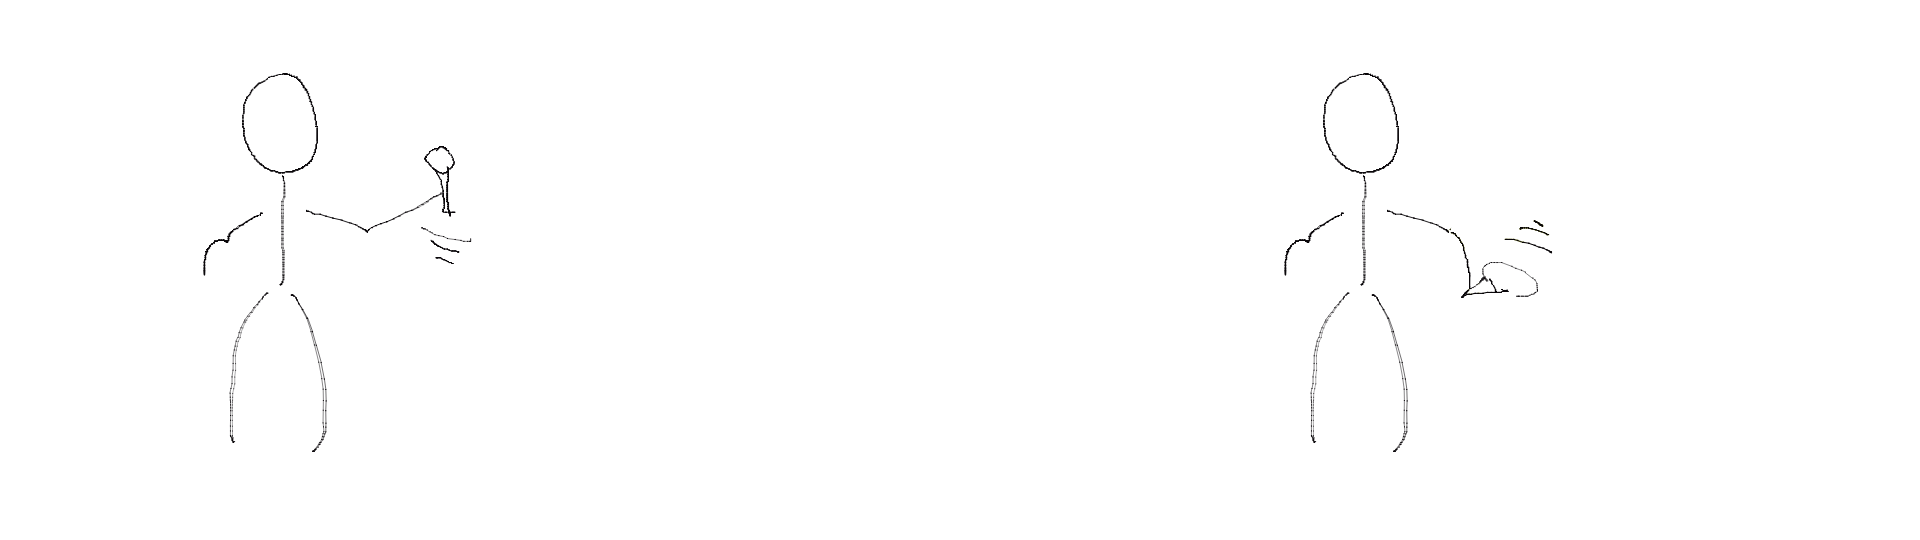
\includegraphics[width=\textwidth]{_raw_resources/offsets/motion-difference.png}
	\caption{Example of the visual difference between the (left) real world 
	capture and (right) the received imagery.}
	\label{fig:offsets:example}
\end{figure}


To mitigate this offset there are two options:

\begin{my_list}
	\item Change the camera setup - in example for a webcam, which usually has 
	a lower offset, ranging between 5 - 250ms. That would degrade the image 
	quality significantly but would enable better rendering conditions inside 
	the engine.
	\item Capture virtual images of the 3D environment and keep them on the GPU 
	until a real world video frame is loaded onto the GPU for usage. This keeps 
	the image quality but needs significant effort to reproduce the rendering 
	conditions at the engine time when a video frame was taken. 
\end{my_list}

The proposed solution uses the second option, since it is able to minimize any 
kind of offset between render image and a video stream, the setup can stay 
dynamic and it is little to no difference by switching to a webcam-integrated 
solution, than an encoding box and the resulting displayed image has only 
non-significant differences to the former variant.

\begin{figure}[htb]
	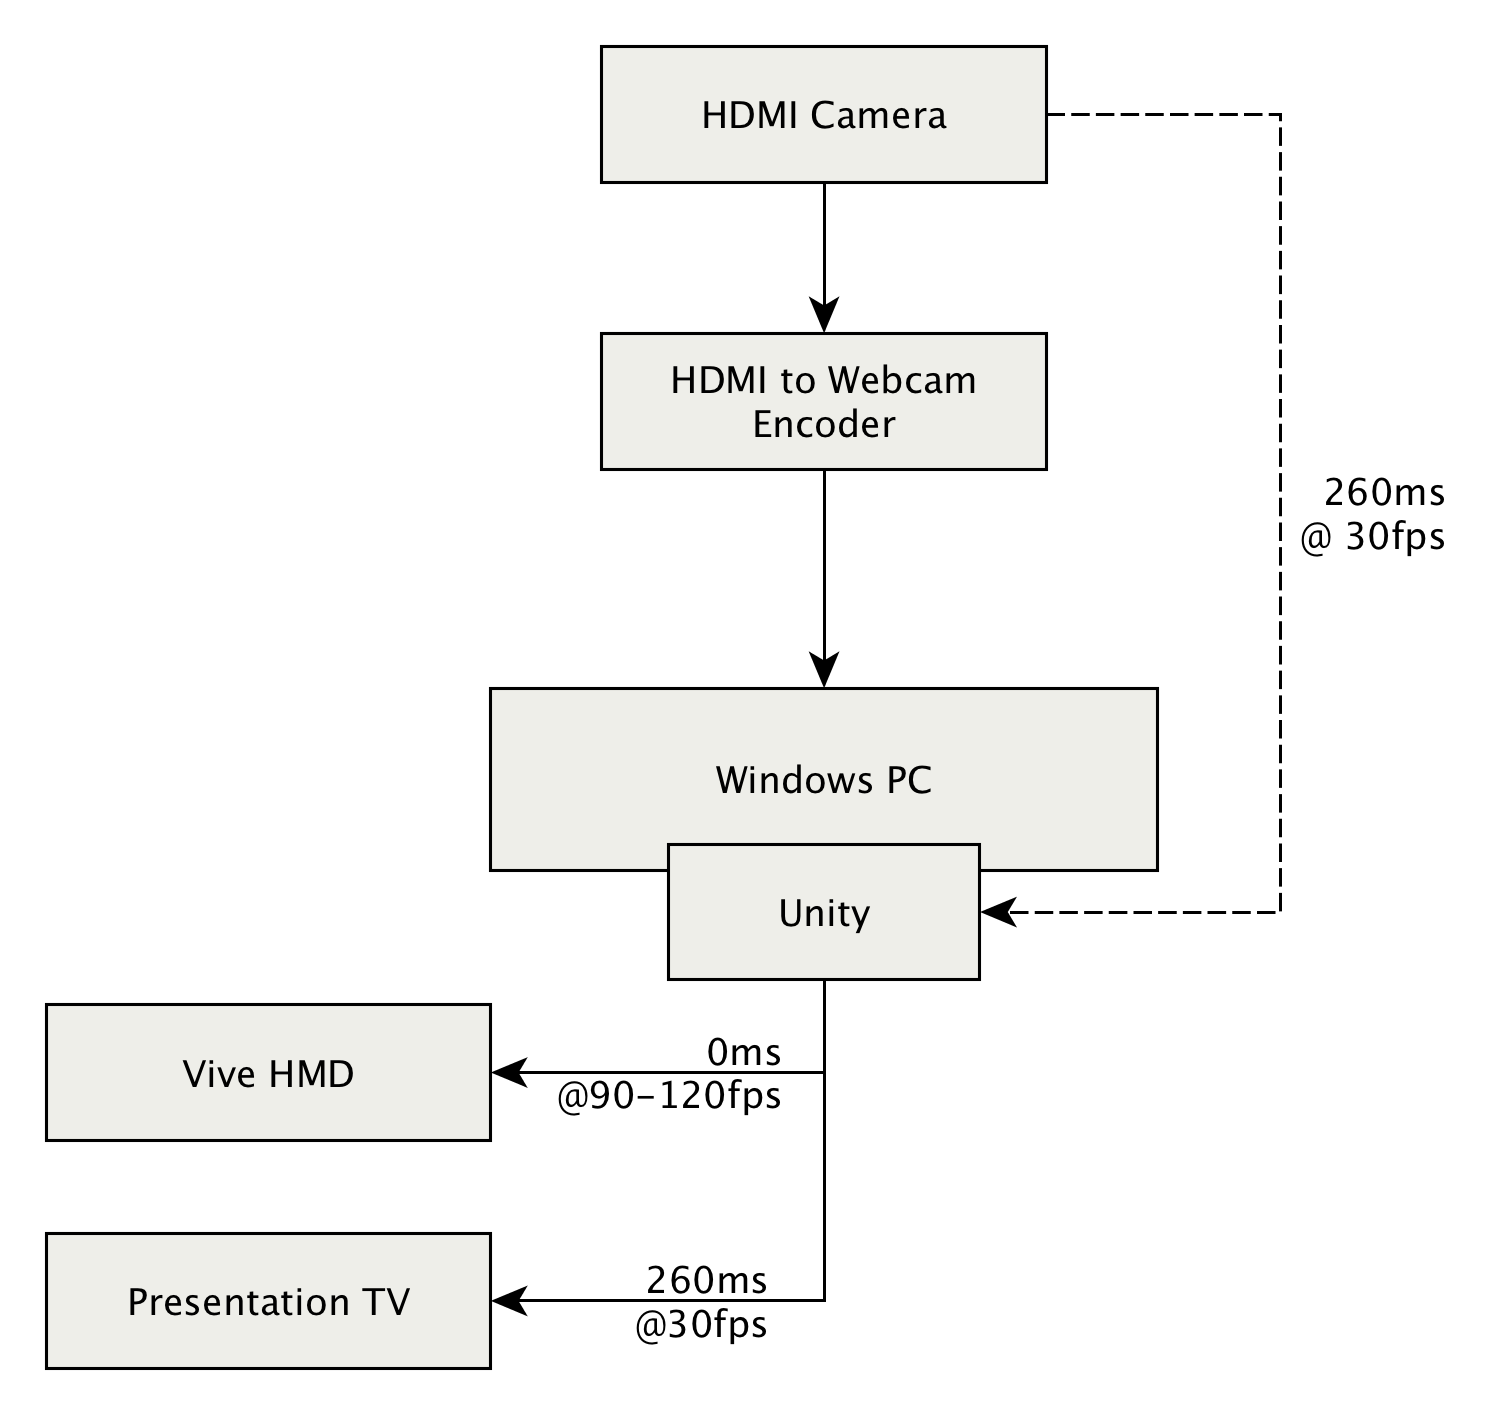
\includegraphics[width=\textwidth]{gfx/FPS-Timing-Components.png}
	\caption{Components in considering timing offsets}
	\label{fig:offsets:components}
\end{figure}

Based on the component diagram \ref{fig:offsets:components} there are two 
important takeaways: The time offset between camera to Unity and the TV and 
Vive HMD framerate differs. At time of writing Unity does not support dynamic 
framerates on multiple viewports. It is possible to manually initiate a render, 
however, this causes the render loop to mistime and yields to inconsistent 
frame timings inside the HMD and is no different between the average GPU load 
to display the presentation TVs viewport.
\newline
To conclude: The software has to store a set amount of \gls{framebuffer}s and 
cycle them at the right frame to guarantee minimal delays between camera and 3D 
environment.
\newline
Noteworthy is that the render loop can be 45 or 90 fps, depending on scene 
complexity, slow system performance or - in case of Unity - garbage collection, 
that could halt the engine for a significant amount of time. To account for 
this a strategy is needed in which Unity's \code{Time.deltaTime} property is 
used, which describes the time between last and current frame.

\subsection{Framebuffer Swapper implementation}

Unity has a well engineered engine loop, where it can perform different 
operations in specific steps of engine execution. For more detail about Unitys 
core engine loop, there is a flowchart in the Appendix \ref{app:engineloop}. As 
initial data needed is \code{cameraFPS}, \code{cameraOffset} and 
\code{Time.deltaTime}. From there it is possible to calculate the remaining 
data for this algorithm:

\begin{lstlisting}
	frameWindow = 1.0 / cameraFPS;
	delayCnt = cameraOffset / frameWindow;
	frameDelay = (int) delay * frameWindow;
	fractionDelay = delay % (1 * frameWindow);
	innerTimer = 0.0;
	absoluteTimer = 0.0;
	while(true) {
		innerTime += Time.deltaTime;
		absoluteTimer += Time.deltaTime;
		localTime = innerTimer - fractionDelay;
		if(localTime < frameWindow ||
		   absoluteTimer < initialDelay) {
			continue;
		}
		
		innerTimer %= frameWindow;
		absoluteTimer %= (1f + initialDelay);
	}
\end{lstlisting}

\todo[inline]{this code listing is the wrong one :( - also I am missing 
representative material why we need to mitigate the latency mitigation}

In Unitys' case a framebuffer is called \gls{render texture} and allows for 
either data or depth buffer access, where a framebuffer would allow for 
simultaneous access.

\subsection{Double Access Ringbuffer}

To spare memory overhead it is possible to reuse previously allocated 
\code{RenderTexture}s by overwriting the second oldest \code{RenderTexture} and 
compositing a mixed reality image with the oldest \code{RenderTexture}(see 
Figure \ref{fig:offsets:ringbuffer}).

\begin{figure}[htb]
	\centering
	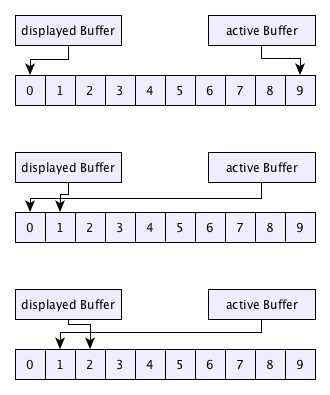
\includegraphics[width=.5\textwidth]{gfx/ringbuffer_schematics.png}
	\caption{Schema of an the ringbuffer}
	\label{fig:offsets:ringbuffer}
\end{figure}

To accommodate for that behavior we have to simply write into the current index 
and display the frame on its next index. After that step taken we increment by 
one. This way we’re overwriting the oldest seen RenderTexture and show the one 
written after it.

\begin{lstlisting}
class DoubleAccessRingBuffer<T> {
	public int bufferSize;
	private List<T> buffers;
	private int index;
	
	public DelayedRingBuffer(int bufferSize) {
		this.bufferSize = bufferSize;
		index = 0;
		buffers = new List<long>();
		RebuildBuffers();
	}
	
	public T[] Next(T writeTo, T display) {
		index %= buffers.Count;
		T writeTo = buffers[index];
		T display = buffers[
			(index + 1) % buffers.Count
		];
		if(bufferSize != buffers.Count) {
			RebuildBuffers();
		}
		index++;
		return new T[]{writeTo, display};
	}
	
	void RebuildBuffers() {
		buffers.RemoveAll(_ => true);
		for(int i = 0; i < bufferSize; i++) {
			buffers.Add(new T());
		}
	}
}
\end{lstlisting}

\todo[inline]{Needs "real" pseudo code, rather than implementation}